% This file should be replaced with your file with an thesis content.
%=========================================================================
% Authors: Michal Bidlo, Bohuslav Křena, Jaroslav Dytrych, Petr Veigend and Adam Herout 2019

\chapter{Introduction}
The majority of today's software applications feature a graphical user interface(GUI). The term GUI application or GUI software is used for an application that uses GUI as a primary interface for interaction, also called reactive systems. The visible GUI structures are made from the components, these components accept sequences of user events that alter the state of the software. The modification of state may or may not include a change to the visible GUI itself. 

The testing of GUI software involves executing events belonging to GUI components and monitoring resulting changes to the program state. GUI test cases consist of event sequences as an input and some indication of a program's state. An indicator can be GUI state, memory state, error log, output log or any other indicator of runtime application state. GUI testing represents a form of system-level testing for GUI software. GUI test cases actually tests much more than the code only associated with GUI, as the events execute underlying non-GUI code. In cases where an application has no non-GUI interface, the GUI testing is the only possible form of system-level testing. This makes GUI testing a critical part of testing for any GUI software.

The size and complexity of modern GUIs, in terms of components and events that may be executed on them, exceed the practical limits of exhaustive and analytical approaches to testing. The number of possible test cases for GUI increases exponentially with the number of events per test case.\cite{NguyenBao2014Gait}

The goal of this work is to design and implement a tool for generating tests for GNOME desktop applications using AT-SPI metadata created as a by-product of an architecture supporting assistive technologies.

The first chapter is dedicated to methods and practices for testing graphical user interfaces. From advantages and disadvantages of the random input testing and manual testing methods to various tools used for a development of automated test cases based on image recognition and record and replay technique. Further discussion is dedicated to a technique named Model-based testing. The technique is presented with approaches used for automated test generation. 

The next chapter is focused on the architecture of accessibility technology for GTK3/GNOME applications, including libraries, tools and applications for debugging. Further analysis contains description of accessible objects and their properties. A set of certain properties describes a state of an application, the state can be changed through various actions executable on accessible objects. After the initial analysis, the focus will be placed on evaluation of accessibility and its usage for designing automated test cases. Limitations and encountered problems are discussed with proposition of additional technologies that should provide additional level of verification. Namely, an image matching algorithms provided by an open source library OpenCV and Optical Character Recognition method designed for extraction of a text from images.

Finally, the proposed solution is being discussed. Starting with the extraction of actions and states from a running application with enabled assistive technology to the process of generation of test case files, which will be prepared to be executed repeatedly. Methods for Code coverage analysis will be discussed as well. 

\chapter{Testing Graphical User Interfaces}
Graphical user interface (GUI) is an interface that takes advantage of the computer's graphics capabilities to make software easier to use.\cite{guidefinition} Graphical applications are developed using sets of windows and widgets. A widget represents a graphical element describing certain behavior and functionality. User interaction with widgets is generating various events allowing them to perform tasks in different ways while achieving the same goal. Although they improve usability and flexibility, they also represent a challenge for software testing as testers have to decide whether to check all sequences of events or only a subset. The effort required to test the GUIs can be reduced with automated software testing. Even though there was significant progress made in automated testing tools over the last decade, manual testing is still the most common technique in practice. However, with a proper automated GUI testing process, more test cases can be executed regularly and more faults can be found within less time.\cite{patternbasedtesting} Automation and CI-CD system play an essential role in regression testing, especially in the test development phase, when software changes are more frequent. Generally, building GUI test cases involves selecting sequences of GUI events and describing the expected state of the program after event execution.\cite{NguyenBao2014Gait}

Next several sections are dedicated to various testing techniques used to test GUIs. Variations of both manual and automated testing are discussed, followed by examples of tools using them. Throughout the chapter a tested application will be referred to as a system under test (SUT).

\section{Random Input Testing}
The Random input testing technique is also referred to as stochastic testing or monkey testing. The term monkey is mentioned in any form of automated testing performed without any user bias. This method distinguishes 3 types of monkeys who are testing the application by generating random sequences of events from both a keyboard and a mouse. Dumb monkeys do not have any knowledge about the system, nor its state. They are not aware which actions are legal or illegal. The downside is that they cannot recognize a failure when they encounter one. Their only goal is to crash the SUT. Another group, referred to as semi-smart monkeys, can recognize a bug when they see one. The last group are smart monkeys, who have certain knowledge about the application they are testing, obtained from a state table, or a model of SUT. On the other hand, smart monkeys are the most expensive to develop. Despite the fact that a random testing tool has a weak coverage, Microsoft has reported that 10-20\% bugs in their software were discovered by this method.\cite{nyman}

\section{Manual Testing}
In general, high-level GUI and acceptance tests are being performed manually. Those practices are often inefficient, error-prone, and tedious. Test development tends to be delayed and executed in a hurry during late development stages. Manual tests are pre-defined sets of steps performed on a high level of system abstraction to validate the system against the required specification. However, software is prone to changes, and therefore it needs to be tested regularly against regressions. This leads to excessive costs, since testers have to continuously re-execute test plans throughout development stages.\cite{guitesting}

\section{Test Automation and CI/CD}
Automated testing solves the major weaknesses of manual testing. The process of automating software testing is similar to a software development process. The goal is to reduce the need for human involvement in repetitive or redundant tasks. List of tests that can be automated include\cite{ci_tests}:
\begin{itemize}
    \item functional - testing that operations perform as expected
    \item regression - testing that the behavior of the system has not changed
    \item exception or negative - forcing the error conditions on the system
    \item stress - determining the absolute capacities of the application and operational infrastructure
\end{itemize}

Implementation of the test automation leads to practices like continuous integration (CI) and continuous delivery (CD). Continuous testing goes beyond the test automation and bring the testing as close to the software development as possible.

Continuous integration is a coding philosophy and set of practices that drive the development teams to implement small changes and check the version control repositories frequently. The majority of modern applications require code development in different platforms and tools, thus the team needs a mechanism to integrate and validate the changes. The goal of the CI is to establish a consistent and automated way to build, package, and test applications. With consistency in the integration process in place, teams are more likely to commit code and changes more frequently. This leads to better collaboration and software quality.

Continuous delivery starts where continuous integration ends. CD automates the delivery of applications to selected infrastructure environments. Therefore it performs necessary calls to predefined sets of services to ensure that applications are deployed.

The common goal for CI/CD is to deliver quality software and code to users. Continuous testing is often implemented as a set of automated regression, performance, and other tests that are executed in CI/CD pipelines. Automated testing frameworks help quality assurance engineers define, execute and automate various types of tests that can help development teams know whether a software build passes or fails. The most CI/CD tools let developers kick off a build on-demand, triggered by code commit in the version control repository, or on a defined schedule. The regression tests are an essential part of the CI/CD pipeline that directly informs developers about the effects of their changes on previously tested and stable functions of the application.\cite{CI}  

\section{Black Box Testing}
The technique handles the software as a black box. A tester has no knowledge about the implementation of the software. The design of the test cases is only based on the specifications and requirements. Tests usually involve a set of both valid and invalid inputs with predictable outputs. Black box testing plays a significant role in testing as it is evaluating the overall functionality of the software.\cite{white_black}

\section{White Box Testing}
The design of test cases depends on the implementation of the software entity. White box testing is focused on internal logic and structure of the code, testing the software from the developer's perspective. The design of test cases requires full knowledge about software's sources, thus allowing to possibly test every branch in the code. Test cases are usually written as unit tests, system or integration tests. Tests are suitable for execution during the development and testing of the finished product as well.\cite{white_black}

\section{Record/Replay and Scripting Tools}
To mitigate the mentioned concerns and increase the quality of software, automated testing has been proposed as a solution. A considerable amount of work has been devoted to high-level test automation, resulting in Record and Replay techniques. Tools are continuously recording the coordinates and properties of GUI components during manual user interaction. Obtained recordings can be played back to emulate user interaction and validate the correct state of the system during the regression testing. These techniques have also certain limitations, which is typically sensitivity to GUI layout changes and code changes. The changes are forcing testers to repeat the recording processes and therefore, they cause additional costs by maintaining automated tests.\cite{guitesting} 

An example of this category of tools is the open-source project GNU Xnee\footnote{\url{https://xnee.wordpress.com/}}. The project consists of a library and two applications. Test automation is one of the several use cases for this project. However, the project is limited to X11 display environments.\cite{xnee}

A similar approach for testing is presented by scrip-based frameworks. These frameworks provide scripting languages to control the GUI. Instead of performing tests manually, testers are writing scripts to automatically interact with the GUI. Scripts contain some assertions to check whether the application executed sequence of events correctly. Violation of assertions during the test results in test case failure. Examples of these tools used widely across the industry are: JFCUnit\footnote{\url{http://jfcunit.sourceforge.net/}} as a tool for testing Java Swing applications. Selenium\footnote{\url{https://www.selenium.dev/documentation/en/}} as a project with a range of tools and libraries that enables automation of web applications. Robotium\footnote{\url{https://github.com/RobotiumTech/robotium}} test automation framework, which allows to write automatic black-box tests for the UI of Android applications. And finally SOAtest\footnote{\url{https://www.parasoft.com/soatest/web-ui-testing}}, with support of integration testing for web applications by capturing user interactions directly in the browser without requiring any scripting.\cite{NguyenBao2014Gait}

\section{Random-walk Tools}
Unlike previously mentioned script-based and capture/replay tools, random-walk tools do not generate test cases. They just randomly walk through the GUI and randomly execute all events they encounter. These tools are easy to use and may find bugs by using unexpected combinations of events. On the contrary, they can reveal only specific tool-supported error events (e.g., crashes, timeouts, permission errors). Tools using this technique are Android Monkey\footnote{https://developer.android.com/studio/test/monkey} and GUIdancer\footnote{https://testing.bredex.de/}.

\section{Solutions Based on Image Recognition}
This category of solutions is often being referred to as Visual GUI Testing. It is an emerging technique combining scripting languages with image recognition. The image recognition allows us to test various systems regardless of their implementation, operating systems, or even platform. Tools are providing support for emulating user interaction with the bitmap components (images, buttons) shown to a user on the screen. The biggest limitation of solutions based on the image recognition is that they are not suitable for highly animated GUIs.\cite{guitesting}. There is also a considerable amount of work required for test maintenance, mostly caused by design changes of widgets throughout the development.   

There are several examples, including the open-source tools Xpresser\footnote{\url{https://wiki.ubuntu.com/Xpresser}} and Sikuli\footnote{\url{http://www.sikulix.com/\#home1}}. The~Xpresser is a python module that works with a directory of images containing cropped images of widgets. Once the image matching algorithm identifies a location of cropped image on the screen, an intended action can be performed on given coordinates.\cite{xpresser} The~Xpresser is mostly used for building automated test cases for Linux distribution Ubuntu.

\section{Model-based Testing}
Model-based testing (MBT) is a software testing technique where test cases are generated from a model that describes functional aspects of the SUT. It allows checking the conformity between the implementation and the model of the SUT, with a more systematic and automatic approach in the testing process. The test generation phase is based on an algorithm that traverses the model and produce test cases suitable for automatic execution.\cite{embedded}

\subsection{Existing solutions}
TEMA toolset is an MBT framework developed for smartphone applications. Testers have to manually create a two-tier model consisting of two state machines, called action and keyword machines. Those machines represent the GUI at design and implementation levels. The method generates design-level test cases by traversing the action machine, afterward the keyword machine is used to transform design test cases in the executable ones.\cite{TEMA}

Another approach was introduced GUITAR\cite{NguyenBao2014Gait} framework for automated GUI testing. GUITAR can be divided into the following parts:
\begin{enumerate}
    \item GUI reverse engineering
    \item automated test case generation
    \item automated execution of test cases
    \item support for platform-specific customization
    \item support for addition of new algorithms as plugins
    \item support for integration into other test harnesses and quality assurance workflows
\end{enumerate}

The first step contains a reverse engineering process. A structural GUI model of an application under test is extracted from the run-time state of the application. This process involves automatic execution of an application, where the tool called Ripper is used to discover as much as possible about the application. The application's window and widgets are discovered in a depth-first manner. The Ripper extracts properties of widgets such as position, color, size, and enabled status, followed by information about events and results of event execution. The depth-first traversal terminates when all GUI windows are covered. The problem with this heuristic is that it would hypothetically contain an infinite number of ways to interact with non-trivial GUI applications. At the end of the process, the Ripper stores the extracted structural information about the GUI in a data structure called GUI Tree, in XML format.

To complete the reverse engineering process, a tool called Graph Converter provides a platform-independent framework to convert the GUI Tree model into a graph, representing relationships between events in the GUI of the application. The result is an Event-flow Graph used for test case generation.
An EFG is a directed graph representing all possible event interactions on a GUI. Each node represents a GUI event. An edge from node \textit{v} to node \textit{w} represents a \verb|follows| relationship between \textit{v} and \textit{w}, indicating that event \textit{w} can be performed immediately after event \textit{v}. An EFG is analogous to a control-flow graph, in which vertices represent program statements and edges represent execution flows between the statements.

Then in step 3, test cases are automatically generated based on the EFG. Therefore, the GUI test generation problem is reduced to a problem of graph traversal. Therefore, any graph traversal algorithm can be used for test generation. 

\subsection{Other GUI model representations}

Other than the EFG approach is labeled state transition systems, action words, and keywords to describe a transition model as the Labeled Transition System(LTS). The LTS consists of a set of states and a set of transitions among those states. Action words describe user events with a high level of abstraction and keywords correspond to keypresses and menu navigation. The goal is to provide abstract tools, so test cases can be designed even before the system implementation. 

One of the most used solutions for designing models are Finite state machines. This approach is also solving certain limitations of the EFG approach. The EFGs are not able to model certain scenarios where GUI objects are modified dynamically. A case where the visibility of the GUI object depends on another object's state is a good example. Additionally, state-charts models can be used for both modeling and generation of test cases for GUIs.\cite{patternbasedtesting}


\chapter{Accessibility Architecture}
Accessibility in general is a technology that helps people with disabilities to participate in essential life activities. Considering the accessibility as a part of the GNOME desktop, it includes libraries and development tools allowing users with disabilities to use other options of interaction with the GNOME desktop environment. Those options include voice interfaces, screen readers, and other alternative input devices.\cite{gnomeADG}
\section{The Accessibility Toolkit (ATK)}
Assistive technologies are receiving information from the Accessibility toolkit (ATK), which offers built-in APIs for all GNOME widgets. ATK provides a set of interfaces that are required to be implemented by GUI components. Therefore, assistive technologies can automatically read most of the labels on screen without any extra efforts made by developers. The interfaces are toolkit-independent, meaning that their implementation could be written for many widgets, including widgets from frameworks such as GTK3\footnote{https://www.gtk.org/} and Qt\footnote{https://www.qt.io/}.
\section{GNOME Accessibility Implementation Library (GAIL)}
The majority of GNOME applications are written in GTK3 framework. The framework provides a dynamically loadable module named GAIL implementing ATK interfaces for all GTK3 widgets. Once the module is loaded at runtime, the application is fully capable to cooperate with ATK without any further modifications.
GNOME desktop does not load accessibility support libraries by default, it has to be enabled by setting a special \texttt{gsettings} key, which can be achieved either by \texttt{dconf}\footnote{https://wiki.gnome.org/Projects/dconf} editor or via \texttt{gsettings} command-line utility using a terminal application:

\begin{lstlisting}[numbers=none,caption={Enabling accessibility via gsettings command},label={gsettings}]
gsettings set org.gnome.desktop.interface toolkit-accessibility true
\end{lstlisting}

Additional configurations may be required for applications written in other frameworks such as QT or Java. Furthermore, implementations of other assistive technologies might be too application-specific or use various techniques like OS event snooping, etc. Compared to GNOME Desktop, all information required by assistive technologies (AT) is passed from the GNOME Accessibility Framework to a toolkit-independent Service Provider Interface (SPI). The SPI is a key component providing a stable and consistent API for screen readers, magnifiers, etc. Accessibility support is relying on per-toolkit implementation (GTK3, QT, Java) and its APIs exported through relevant bridges to unified AT-SPI interface as described in Figure \ref{ATSPI_architecture}.

% Make sure that every image is referenced at lease once with proper positioning
\begin{figure}[hbt]
	\centering
	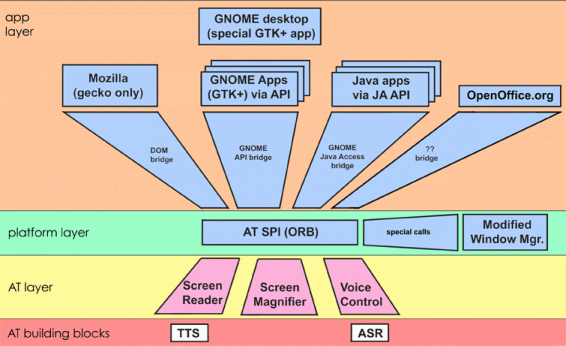
\includegraphics[width=1\textwidth]{obrazky-figures/GNOME_desktop_Accessibility.png}
	\caption{GNOME Accessibility Architecture overview\cite{gnomeADG}}
	\label{ATSPI_architecture}
\end{figure}

The widget is accessible, if a developer uses any GTK3/GNOME widget and follows the general accessibility guidelines\footnote{https://developer.gnome.org/accessibility-devel-guide/stable/gad-coding-guidelines.html.en} with properly implemented ATK interfaces. Considering that the stock GTK3/GNOME toolkit widgets have implementations of these interfaces provided, new widgets will inherit the functionality and gain suitable accessibility support as well. The default implementation of ATK interfaces might be altered by applications, as developers can enrich their descriptions of widgets and improve the overall user experience in special cases, e.g. when a widget is used for some less expected purposes or the default description is too general. The ATK provides a set of functions to achieve this along with the ability to make any custom component accessible\footnote{https://developer.gnome.org/accessibility-devel-guide/stable/gad-custom.html.en}.\cite{accessibleWidgets}

\newpage
\section{Library Pyatspi}\label{library_pyatspi}
Package pyataspi is a Python wrapper around AT-SPI's C implementation, which loads the Accessibility typelib and imports the classes implementing AT-SPI interfaces.\cite{pyatspi}

AT-SPI exposes applications as a tree of widgets, starting with a root element where every sub-element represents one running application on the GNOME desktop. Each application has zero or more child elements, each child is distinguishable by its position in the tree and several object properties. Some of these properties are encapsulated inside the accessible object and their values must be obtained through corresponding methods, so-called getters. A small set of properties are described in the following list:
\begin{itemize}
    \item \textit{name} - a string value, for most widgets contains text identical with a text label visible on widget
    \item \textit{roleName} - a string value, specifies the widget type, available via \textit{getRoleName} method
    \item \textit{childCount} - an integer value, a number of sub-elements 
    \item \textit{actions} - a list of strings, contains available actions which can be performed by the ATK
    \item \textit{visible} - a boolean value, indicated that object is visible to the user
    \item \textit{showing} - a boolean value, object is rendered
    \item \textit{text} - a string value, mostly used in input fields or widgets containing plenty of text
    \item \textit{description} - a string value, contains special widget description for users
    \item \textit{position} - an integer tuple, x, y coordinates on the screen (might be related to other component)
    \item \textit{size} - an integer tuple, shows theight and width of a widget
\end{itemize}

Additionally, elements can be linked together in other useful ways (except parent-child relationship where labels are linked with widgets like text fields, check boxes, combo boxes, etc. These labels are making widgets easier to find or interact with. Other advantageous properties like \textit{showing} or \textit{visible} can be used to decide whether elements are hidden from the active screen area, thus they are not available for interaction. Specifying a \textit{roleName} allows the categorization of widgets which is useful for identification of category-specific methods, e.g. selecting values in radio buttons, selecting options in combo boxes, or a simple click method on push buttons. Access to this functionality is focused in a singleton object named \textit{registry} that provides services for subscribing to specific events and generating events from mouse or keyboard on demand.

Library pyatspi is an open-source project available for most Linux distributions via distro specific packaging services (package named \textit{python3-atspi}) or is available to be built from its sources\footnote{https://gitlab.gnome.org/GNOME/pyatspi2}.

\section{Exploring and Debugging The Accesibility}
Currently, there are several tools available for exploration and debugging accessibility features not only on the GNOME desktop. 
\subsection{Library Dogtail}\label{sniff_accerciser}
Dogtail is an open-source GUI test framework written in Python implemented as a library around pyatspi. Several modules implements a higher level of API to simplify work and interaction with accessible objects during test development. The tool offers less complex functionality, containing tree view of objects with their basic attributes\cite{dogtail_doc}. Package dogtail also includes a GUI tool Sniff (AT-SPI Browser on Figure \ref{sniff}), similar to the Accerciser application described in the next section. The most important dogtail modules are described in several next paragraphs.

\begin{figure}[h]
	\centering
	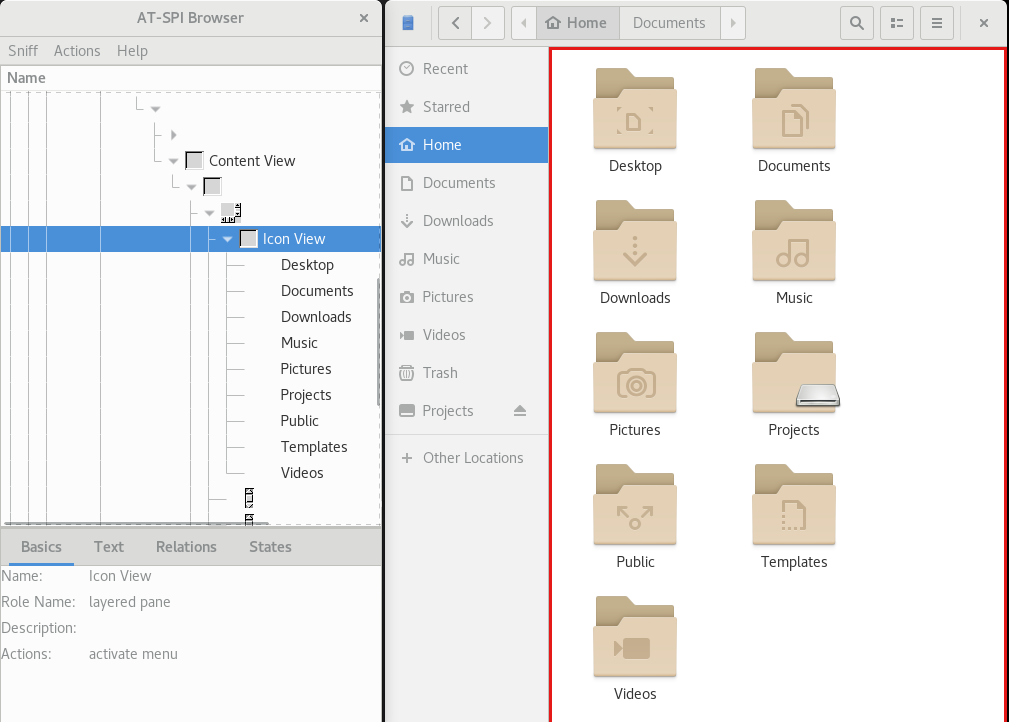
\includegraphics[width=1\textwidth]{obrazky-figures/sniff.png}
	\caption{Sniff utility (AT-SPI Browser), highlighting Icon View area in Nautilus File Manager, Screenshot taken from Red Hat Enterprise Linux 8.2}
	\label{sniff}
\end{figure}

The module \textit{tree} contains the most important class \textit{Node}, instances of the class represent elements of the desktop user interface. All elements are gathered to the tree structure, representing all applications starting with the root element (desktop). The class is implemented as a mixin for Accessible and various Accessible interfaces and is an important unit for its subclasses, namely \textit{Application}, \textit{Root} and \textit{Window}. The Node class also implements methods used for search of nodes in the tree based on certain criteria. A lambda expression can be passed to methods \textit{findChild} and \textit{findChildren} as argument named \textit{pred}. The lambda expression can contain any properties that uniquely identify nodes, including \textit{name}, \textit{roleName},  \textit{showing} and \textit{visible}. The class also contains action methods that can be performed on nodes without importing other action modules. Verification and identification of shown nodes are easier thanks to the method named \textit{blink}. Once the method is called on a certain element, the element is highlighted on the screen for several seconds. This functionality is also part of the Sniff tool where an element is highlighted after it is selected in the displayed tree.

The module \textit{dump} contains only one method with the same name, the method returns a string describing the tree of nodes which is useful for python/ipython console debugging.

Finally, the module \textit{rawinput} contains the implementation required for generating events from both keyboard and mouse. More complex events simulating keyboard shortcuts, mouse gestures, and drag and drop operations are implemented as well.  

 Testing Dogtail has proven availability for many Linux distributions through their package repositories, specifically Fedora 32, Red Hat Enterprise Linux 8.2 and Manjaro 18 with GNOME 3.34 (Archlinux). It is also available as a Pypi Python package and according to information in it's official Gitlab repository should work not only for GTK3 application but also for application written in QT and KDE. 
 
 Dogtail testing reveals also some minor problems which might occur during the test development. To be more specific, there are know cases in which the coordinates of a node were not reported correctly. Most of the items labelled with a \textit{roleName} panel and list list box are missing their \textit{name} labels. Those items are not as important for users as they don't contain any visible text, nor an action to interact with. The purpose of those items is to serve as a wrapper for other elements and group them together in an element tree. Further testing discovered non-accessible menu\footnote{https://bugzilla.redhat.com/1723836} or nameless menu button\footnote{https://wiki.gnome.org/Apps/DiskUsageAnalyzer}. So once an action needs to be dispatched on such element, the identification has to be done either through a parent element or a sibling element. Additionally, execution of a mouse event will require an offset calculation to specify the correct element position on the screen.
 
 So to conclude this chapter, dogtail is a powerful tool for the development of automated test cases in the GNOME3 environment. On the other hand, it contains discussed limitations and flaws. Those limitations must not come from the dogtail itself. They are either accessibility bugs or bugs in the GTK3 framework (non-accessible menu).  

\subsection{The Accerciser}
The accerciser is an interactive accessibility explorer developed in Python. It provides a well-arranged graphical frontend for the AT-SPI library, hence it can inspect, examine and interact with widgets. It also serves as a verification tool for developers, to check that their applications are providing correct information to assistive technologies and automated testing frameworks. The~Figure \ref{Accerciser_img} demonstrates the interface with extended features and functions when compared to Sniff. The default interface has three sections, a~tree view with the entire hierarchy of accessible objects and two optional plugin areas. The~Accerciser has an extensible, plugin-based architecture. Most of the features available by default are provided by plugins discussed in the next several paragraphs.

The Interface Viewer plugin is an explorer of AT-SPI interfaces provided by each accessible widget of a target application. Once an item is selected, its interfaces are shown with a list of sensitive methods. The majority of methods are executable. The list contains methods for interaction with an object and various methods for obtaining more information about the object. The Accerciser offers an exploration of the following interfaces:
\begin{itemize}
    \item Accessible - shows child count (number of child widgets), description, states, relations, and other attributes
    \item Application - if implemented (not mandatory), it shows application ID, toolkit and version
    \item Component - shows item's absolute position with respect to the desktop coordinate system, the relative position with respect to the  window coordinate system, size, layer type, MDI-Z-order indicating the stacking order of the component and alpha
    \item Document - shows document attributes and locale information
    \item Hypertext - shows a list with all item's hypertext links,  including name, URI, start index and end index
    \item Image - shows item's description, size, position and locale
    \item Selection - shows all selectable child items of the selected item,
    \item Streamable Content - shows selected item's content type and their corresponding URIs
    \item Table - shows item's caption, rows, columns, number of selected rows, number of selected columns and for the selected cell, it shows  it's row's and column's header extents  
    \item Text - shows selected item's text content, that can be editable with attributes offset, justification  and possibility to show CSS formatting as well
    \item Value - shows an item's value, minimum value, maximum value, minimal increment for a value 
\end{itemize}

\begin{figure}[H]
	\centering
	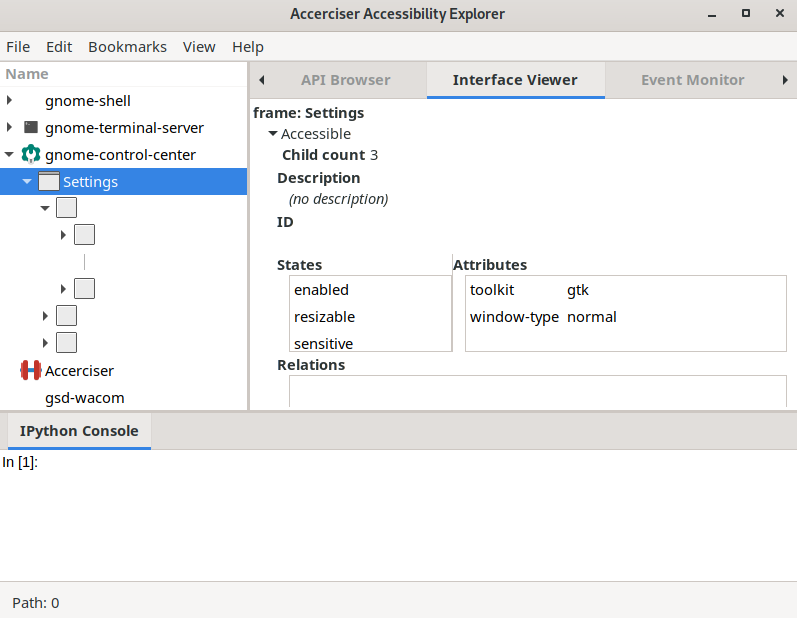
\includegraphics[width=0.8\textwidth]{obrazky-figures/accerciser.png}
	\caption{Accerciser's default configuration, Screenshot taken on Manjaro Linux with GNOME 3.34}
	\label{Accerciser_img}
\end{figure}

The AT-SPI Validator plugin applies tests to verify the accessibility of a target application, the validator will generate the report of the selected item and all its descendant widgets in the tree hierarchy.

The next plugin is the Event Monitor, which displays AT-SPI emitted events including the filter for several different AT-SPI event classes. The plugin has the ability to monitor only events sourced from the selected application or selected accessible (widget). Each event record contains the source and the application.

The Quick Select plugin provides global hotkeys for quickly selecting accessible widgets in the Accerciser's Application Tree View, the selected widget is highlighted in the target application.

The API Browser plugin shows interfaces, methods and attributes available on each accessible widgets of a target application, by default it shows only public methods and properties, private methods and properties are hidden until checkbox \textit{Hide Private Attributes} is unchecked.
 
Finally, plugin IPython Console provides a full, interactive Python shell. The console has immediate access to any selected accessible widgets of a target application. The object currently selected in the tree view is available in the IPython Console under the symbol \textit{acc}, so the plugin provides an easy way to test and debug code used in test cases.    

\section{Covering Limitations of Accessibility and Verification}
As discussed in the aforementioned sections, the information provided by accessibility is not flawless. Therefore, the next couple of chapters are dedicated to the exploration of technologies that might be used to support the accessibility in such cases.

\subsection{OpenCV and Image Matching Techniques}
OpenCV or Open Source Computer Vision Library is a software library that provides optimized algorithms for computer vision and machine learning. According to the official OpenCV webpage\cite{opencv}, the library contains more than 2500 algorithms and it is being developed 
by a vast community of contributors around the world. The library is used extensively bu government institutions, research groups, and companies including Microsoft, Google, IBM, etc. One of the biggest advantages is its native C++ implementation with bindings making the library available in Python, Java, and Matlab and supports Linux, Android, Mac OSX, and Windows. Regardless of Linux distribution, similarly to dogtail, OpenCV can be installed easily via python3 package manager (\texttt{pip}). 

From the rich availability of algorithms provided, the image recognition algorithm can be used to either locate or verify the presence of an element on the screen. This approach would require to have a set of images containing elements prepared in advance, then it can be used to find the image location on the screenshot of the screen taken during a test run. Compared to verification of the node only via accessibility, this approach would also verify that the element is properly rendering on screen and the shown result is an element that is shown to the user. An additional benefit is the verification of text formatting and colors. On the contrary, there this process requires additional manual work of taking images, labeling them, and associating them with certain test scenarios. Count of elements displayed on the screen multiple times creates another parameter that would require manual maintenance. The most common example of such cases are buttons labeled either OK or Cancel as they are used in many applications.

Another possible approach is to use the shape recognition algorithm which can locate shapes like circles, rectangles, and many other common shapes. From the development perspective this would be easier to maintain as there is no requirement for images prepared in advance. Frequent application changes during software development may also cause that tests based on image matching can be easily outdated. This factor forces testers to revisit test suites, therefore the efficiency of automated tests deteriorates. It can also help with the widget location in cases where accessibility is reporting wrong coordinates. On the other hand, locating the right widget in cases when several similarly shaped ones are located on the screen at the same time will yield very inconsistent results.

\subsection{OCR}\label{OCR_section}
Optical Character Recognition or OCR is a method of extracting text from images. One of the available open-source tools is a tool called Tesseract.

Initially, Tesseract development started in 1985 at Hewlett Packard Laboratories but the major breakthrough was achieved in 2006 when the project was open-sourced in cooperation with the University of Nevada in Las Vegas. Since then, the project has been developed under the sponsorship of Google\cite{tesseract_history}.

Usability of Tesseract was increased in version 3.x, supporting a wide range of image formats and gaining the ability to be used in a larger number of scripting languages. While Tesseract 3.x is based on traditional computer vision algorithms, in the past few years methods based on Deep Learning have surpassed traditional machine learning techniques by a vast margin, especially in terms of accuracy in several areas of Computer Vision. Remarkable results were achieved in handwriting recognition. Tesseract has implemented a Long Short Term Memory (LTSM) based recognition engine which is a kind of Recurrent Neural Network (RNN). While this kind of RNN is used to recognize the text of random length, a Convolutional Neural Network is used just for recognition of single character. Version 4 provides both legacy OCR engine and new LSTM engine which is enabled by default.\cite{tesseract}

Tesseract can be used as a command-line tool, integration in development is possible via Tesseract's API available in python or C++. Setup on Linux or other platforms may differ but the process is accurately described in Tesseract's wiki\footnote{https://github.com/tesseract-ocr/tesseract/wiki}, with the last resort solution - building it from its sources.
The setup process includes installation of the \texttt{tesseract-ocr} package itself, \texttt{pytesseract} python bindings installable via python's package manager pip, and Tesseract's language pack with trained data for English language (version 4.x supports 130 languages\footnote{https://github.com/tesseract-ocr/tesseract/wiki/Data-Files\#data-files-for-version-400-november-29-2016}). 

Tesseract's OCR engine works best when used with images containing black text on white background in a common font. Text should be approximately horizontal with the height of at least 20 pixels. Surrounding borders around the text can be detected as some random text. With possibilities of image processing provided by OpenCV, the image quality in some cases needs to be improved before applying text detection methods.The  Most common image preprocessing methods include inverting images, rescaling, binarisation, noise removal, rotation, border removal, and page segmentation\footnote{https://github.com/tesseract-ocr/tesseract/wiki/ImproveQuality}.
\begin{figure}[hbt]
	\centering
	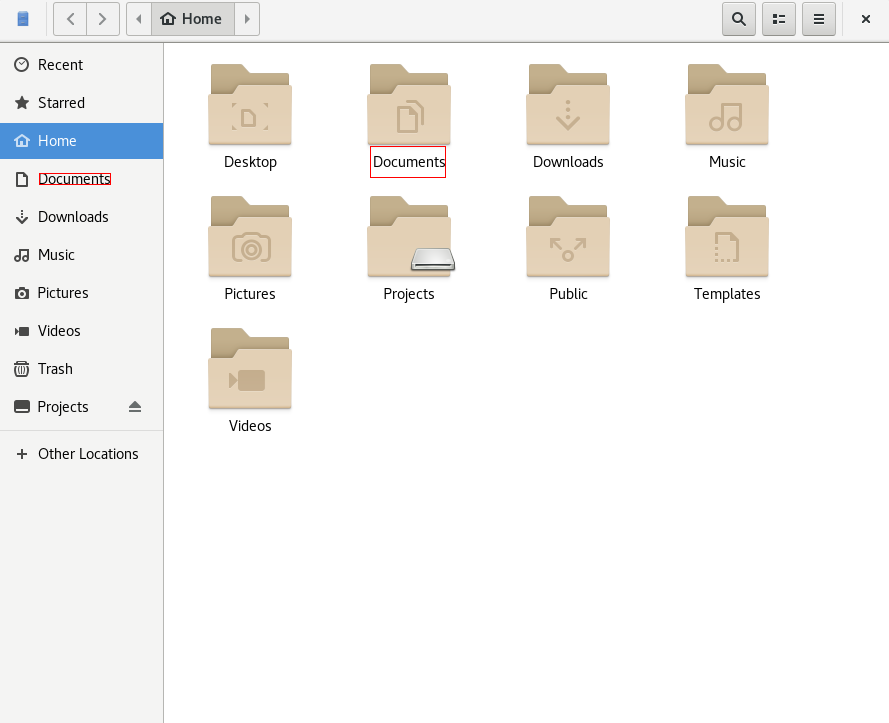
\includegraphics[width=1\textwidth]{obrazky-figures/ocr+nautilus.png}
	\caption{Demonstration of the OCR engine detection for the string Documents in Nautilus File Manager window, Red Hat Enterprise Linux 8.2}
	\label{ocr_nautilus}
\end{figure}
\bigskip

Tesseract's API for python is bundled in a module named \texttt{pytesseract}. The module provides several methods, the most important ones for the of this work are \verb|image_to_string| and \verb|image_to_data|. Both methods have one compulsory parameter which is an image intended for text extraction. An image has to be in a certain format, one of the options is to load the image through OpenCV's \texttt{imread} method. Additional parameters may be applied including language, timeout, and engine configuration\footnote{https://pypi.org/project/pytesseract/}. The first method returns all recognized strings including all whitespaces and other special characters. The second method provides additional metadata about all recognized strings in a form of dictionary-like object. The returned dictionary contains the following lists of properties:

\begin{itemize}
    \item text - string value, may contain a string, special character, one word or line of text
    \item left - integer value, specifies the number of pixels from the left side of the image 
    \item top - integer value, specifies the number of pixels from the top of the image
    \item width - integer value, specifies the width of the recognized string 
    \item height - integer value, specifies the height of the recognized string
    \item the rest are less important values for this work: \verb|level, page_num, block_num par_num|
    \verb| line_num, word_num, conf|
\end{itemize}

Therefore, occurrences of a certain string in an image are filtered and highlighted in every image as demonstrated in Figure \ref{ocr_nautilus} for string \textit{Documents}.

Similarly to OpenCV, Tesseract's OCR engine was tested as an alternative tool for location or verification of widgets that contain text. This method also verifies that the content was properly rendered and is readable for the user. OCR systems have limitations and work with a certain margin of error which is a fact that also applies to Tesseract. Various applications can use different color schemes including background colors and font colors, input fields, and labels. Highlighting elements to perform actions on them can also lead to changes in these conditions. Image preprocessing methods provided by OpenCV can aid in avoiding problems associated with those cases, namely color inversion and binarisation. Those methods would supply Tesseract's engine with an image containing black text and a white background for evaluation.

\section{Conclusion}
This chapter has been dedicated to the Accessibility technologies in GNOME desktop with a deeper look at implementation, libraries, and tools for debugging. Furthermore, technologies that may be able to cover limitations and bugs in accessibility have been evaluated as well. Both OpenCV and Tesseract may help with identification, location, and verification of non-accessible elements in applications. A possible disadvantage is a delay caused by taking and processing screenshots of applications that have to be taken at the right time. OpenCV's image matching algorithm can reliably locate prearranged images of icons, labels, or whole application windows on the screen. Considering the stable application environment with black text on white background in most applications, Tesseract can detect and reliably locate most of the text content on the screen. Other cases can be covered by image preprocessing done again in OpenCV. Both technologies are working with actual application content rendered to users, possibly bringing an additional level of verification. However, the goal of this work is to generate test cases dynamically and preparation of e.g. set of screenshots to verify a proper rendering of icons would violate this effort. A possible solution could be to take screenshots during the test generation process. However, an icon would need to be cropped out from the screenshot, thus relying on the position if the icon reported by the AT-SPI. Therefore, an integration of the Tesseract's OCR would be more beneficial for this project.

\chapter{Proposed solution}
A goal of this work is the development of a tool able to generate automated test cases for GUI applications. The proposed tool should be able to generate test cases mainly from the AT-SPI metadata. The required metadata should be available for a lot of applications, assuming they are using one of the common frameworks (GTK3, QT). However, this tool is targeted on applications for GNOME desktop\footnote{https://wiki.gnome.org/Apps}. A tool will be developed in language Python3, version 3.6.

All applications are open source and are developed by the community of enthusiasts around the GNOME project. Anyone from the community can fix bugs in applications by sending a merge request with fixes, request a new feature, or propose changes with new features. Considering this model of development, there is no future planning nor phase where one can design an abstract model of an application, from which test cases can be derived. Therefore, the solution is based on the derivation of the model from the AT-SPI metadata. 

\begin{figure}[hbt]
	\centering
	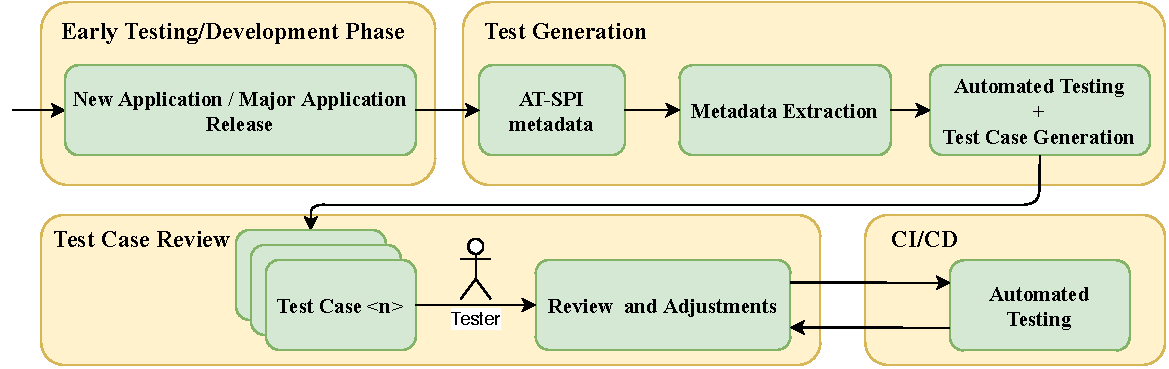
\includegraphics[width=1\textwidth]{obrazky-figures/overview.pdf}
	\caption{Architecture of Proposed Solution}
	\label{Diagram}
\end{figure}

The Figure 4.1 describes an overview of the workflow with the proposed tool. The beginning of the scenario starts with either a newly developed application or a version of an application that contains major changes. The tool should perform an initial exploratory testing of the application based on the extracted model and export those scenarios in the form of behave test scenarios.

From the testing perspective the proposed tool combines several testing techniques. The AT-SPI metadata creates a foundation for a simplified model of the application by partially adapting the Model-based Testing technique. Since the test cases are derived from the model without any knowledge about the implementation of tested applications, the tool resides in the category of Black Box Testing. The presence of the model allows the tool to benefit from the approaches described in the Random Input Testing and Random Walk tools in a more deterministic way. The tool can be characterized as a semi-smart tool as it can detect certain crashes of the SUT during the test generation and immediately report them with a reproducer. The result of the test generation process are test cases that can be adjusted and executed again. The tests are executable in the CI/CD pipeline that can be triggered at any stage of the application development and report the results without manual retesting.

\section{Model Extraction}
The model extraction process relies on AT-SPI metadata which are provided after the start of an application. As mentioned in section \ref{library_pyatspi}, once the application is running, a tree of widgets is exposed and available for interaction. The provided representation of the tree itself is not suitable to be directly used as a model of an application, as the implementation contains several restrictions for purposes of this work.

The first restriction is represented by nodes/widgets with no functionality nor a way of interaction for the user, e.g.: filler, separator, panel, etc. Theoretically, a copy of the three could be created with those nodes filtered out, although in that case the parent-child relationship in the tree needs to be restored accordingly. This is not possible, since the attributes \texttt{children} and \texttt{parent} in \texttt{Atspi.Accessible} object instances are read-only. The tree also contains properties and methods which are available only during application runtime, possibly disallowing access to the properties of an extracted model after application crashes or terminates. 

A solution for those restrictions is a custom implementation of the accessibility tree. First, a custom tree is derived from the original tree. Then, it filters the unusable nodes out, but it preserves the parent-child relationship of the nodes. The custom tree can be taken as a model, that will map the possibilities of interactions available for users working with an application. the model includes every node from the original tree that has an action available that is also executable by AT-SPI. However, the model does not allow the execution of the actions directly, since the generation process requires to run several instances of an application. The instances of accessible objects are valid only for one application runtime. Therefore, several important attributes are extracted in the process, making them available even after the termination of an application instance. These attributes are used for the unique identification of nodes. The attributes give the test generator an ability to match each node from the model to the current application instance exposed by the accessibility. The implementation of the model is presented via class diagram in the Figure \ref{tree_diagram}.

\begin{figure}[hbt]
	\centering
	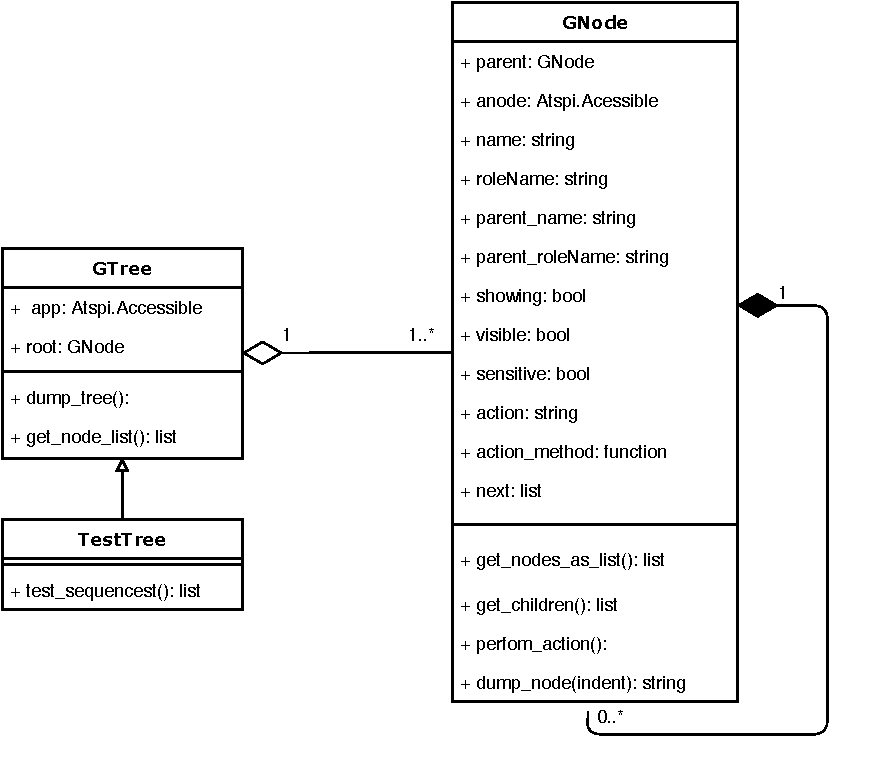
\includegraphics[width=0.8\textwidth,clip]{obrazky-figures/tree_diagram.pdf}
	\caption{Class diagram of a model}
	\label{tree_diagram}
\end{figure}


Starting from the lowest level, an instance of the class \texttt{GNode} represents one node from the tree. Several attributes are copied from the original \texttt{dogtail.tree.Node} instance, including attributes storing pieces of information about the parent node, data describing the state of the node, the list of children, and if available, the name of the action method. The list of children is also composed of instances of the \texttt{GNode} class, so the tree is recreated recursively. Therefore, the model is able to hold all information about tested applications, without relying on their state. An instance of the \texttt{GTree} can represent either a whole application or a smaller part of the application e.g.: a dialog or a menu. As discussed previously, this offline model of the application tree also contains a lot of nodes without the ability of interaction, which needs to be filtered out. Those nodes are identified by the list of \texttt{RoleName}s that are gathered in the separate file \texttt{rolenames.py}. Then, the last class \texttt{TestTree} serves as a wrapper, which filters those nodes and preserves the parent-child relationship. The result of this process is an instance of the \texttt{TestTree} object and it contains only nodes required to generate test cases. 

\section{Test Environment}
Before generation process starts, it is necessary to have an ability to monitor the state of tested applications and have the ability to perform start and stop operations. The test generation process performs various actions available in an application that might change settings or layout of the application. Generation of every test case must start from the same state. A solution is summed up in three steps:
\begin{enumerate}
    \item make sure that the application is not running or force the application to stop
    \item reset the application settings to default state by performing predefined custom cleanup
    \item start a new instance of the application with the default settings.
\end{enumerate}

\subsection{Environment Setup}
The test case generation process depends on the execution of applications in the GNOME Shell desktop environment. The environment contains various features\footnote{\url{https://help.gnome.org/users/gnome-help/stable/shell-introduction.html.en}} like workspaces, notifications, the application grid, the activities overview, and menus, that can be triggered either via mouse or keyboard. Those actions can bring the environment to multiple states. A switch to either the application grid or the activities overview takes the focus from the tested application back to GNOME Shell, thus blocking any further interaction. A notification might collide with the user interface of the tested application and block the execution of an action during the test case. These factors need to be avoided to ensure stability during the test generation and the test execution as well. The setup must be able to recover the environment from potential test case failures and will not influence the execution of the subsequent test cases. 

The required setup for the test execution is implemented in the module \textit{qecore}. The module is designed for test automation of GNOME desktop application and contains various measures designed to avoid occurrences of unintentional environment events and focus on a tested application. The module is bound to the dogtail and it is intended to be used with behave framework.\cite{qecore} 

The test generation process partially relies on the provided setup. However, a different approach is used in terms of monitoring tested applications. For that reason, a custom class \texttt{App} is derived from the qecore's \texttt{Application} class. Throughout the development of the test generator, the implementation of the \texttt{App} class diverged, and the majority of the implemented methods were rewritten. Although, the \textit{qecore's} \texttt{Application} class is still being used for the test case execution. The inheritance acts as a safeguard that makes sure that provided data about a tested applications are sufficient to create an \texttt{Application} instance. Or in other words, it serves as a test that generated tests will be executable before the generation process starts. The relationship between classes is shown in the Figure \ref{test_gen}. Integration with the \textit{qecore} lead to contributions that were delivering minor fixes\footnote{\url{https://gitlab.com/dogtail/qecore/-/merge_requests/24}}\textsuperscript{,}\footnote{\url{https://gitlab.com/dogtail/qecore/-/merge_requests/26}}. Another contribution\footnote{\url{https://gitlab.com/dogtail/qecore/-/merge_requests/25}} submitted an implementation of the new attributes for the \texttt{Application} class to solve the problem with location of desktop files required to test LibreOffice applications.

\subsection{Environment Configuration}
Assurance of compatibility with various applications across the GNOME ecosystem requires, that some metadata describing the tested application has to be provided before the test generation process. The metadata is gathered in a configuration file written in YAML\footnote{\url{https://yaml.org/}} language and only contains the most necessary information required to recognize tested applications. The reasons behind choosing YAML is syntax simplicity and human readability in comparison with e.g. JSON\footnote{\url{https://www.json.org/json-en.html}} or XML\footnote{\url{https://www.w3.org/XML/}}, followed by the reliable support in python provided by library \texttt{pyyaml}.\cite{yaml} The purpose of this configuration file to have one dedicated place as a single source of truth, which means that all application related changes can be edited without any changes in the source code of the test generator.

\begin{lstlisting}[language=yaml,caption={Example of the apps.yaml entry for LibreOffice Start Center},label={apps.yaml}]
libreoffice-startcenter:
  a11y_app_name: soffice
  app_process_name: soffice.bin
  desktop_file_path: /usr/share/applications/libreoffice-startcenter.desktop
  kill_command: "pkill soffice"
  params: "--norestore" # required to avoid unwanted file restore dialogs
  cleanup_cmds:
    - "pkill soffice" # LO required a custom kill cmd
    - "rm -rf .config/libreoffice/*"
  packages:
    - libreoffice
  flatpak: False
\end{lstlisting}

The \texttt{apps.yaml} gathers data about all tested applications. Each application entry starts with an application name on the top level. The application name should be unique as the name is used as a folder name of the generated project. Otherwise, there are no further requirements. Required values may vary per tested application. Some of them might not be necessary for the test generation, although they are required for test execution.
The generated test case require some of the params 
The list items that can be defined for each application includes:

\begin{itemize}
    \item \texttt{a11y\_app\_name} - is the only compulsory item, define a name of the application in the accessibility tree, the value can be found in Sniff or Accerciser as previously discussed in Section \ref{sniff_accerciser}
     \item \texttt{app\_process\_name} - is required if the name of the application process is different than the application name, the value is used to during the cleanup between the executions to make sure an instance of the application has been killed and a next test will use a new one
     \item \texttt{desktop\_file\_path} - required if default qecore's method fails to find the desktop file of an application, the desktop file contains useful data about an application, including a command to run an application from the command line
     \item \texttt{params} - required if the application needs to be run with custom command line parameters, all parameters should be entered in one string with separated with a space
     \item \texttt{cleanup\_cmds} - if provided, contains a list of commands that will be executed after the generation of each test case. Executed commands should always restore the application to its default settings. The commands are also used during the test execution of generated test cases, after finishing each test case. 
     \item \texttt{packages} - required for execution in CI, contains a list of rpm\footnote{https://rpm.org/} packages required to be installed to both generate and execute tests
     \item \texttt{flatpak} - required if tested application is a flatpak
\end{itemize}

\subsection{Flatpak Applications Setup}
Flatpak\footnote{\url{https://flatpak.org/}} is a technology for building and distributing desktop applications on Linux. Flatpak aims to solve the problem with the cross-platform distribution of packages on Linux, thus avoiding problems with different package managers used across Linux distributions. Applications, or so-called flatpaks, are delivered to users regardless of the lifecycle of the underlying Linux distribution. The system implements a set of sandboxing technologies, to isolate flatpaks from each other and the system, thus providing security benefits to users.\cite{flatpak}

The majority of GNOME applications are also available through flatpak. A dedicated flatpak repository \textit{Nightly GNOME Apps} contains the latest development versions of GNOME applications. With Flatpak, those applications are installed alongside their stable versions. This gives us the potential to test the application much sooner before it is released to distributions. This is a benefit behind the integration of flatpak support to this work. The main repository for flatpak applications called Flathub\footnote{\url{https://flathub.org/home}} contains hundreds of applications developed in various frameworks and programming languages. However, the effort done by this work only supports applications developed in GTK as they obtain the accessibility support by design.

There are several differences in the runtime perspective between flatpaks and non-flatpak applications. Each application has a unique name, e.g.: \texttt{org.gnome.gedit}. The unique name is required for every operation executable through the \texttt{flatpak} command-line utility. The utility not only serves as a package manager able to install, remove, downgrade and update flatpaks, it also provides a sandbox to run the flatpaks. Those differences demand certain changes in the runtime used for the test execution and the test generation. 

Considering the test execution, the approach used in the \textit{qecore's} \texttt{Application} class should be suitable for testing flatpaks. However, the initial testing emphasized the previously mentioned differences and it lead to the conclusion that a separate class \texttt{Flatpak} has to be developed to achieve the same goals. The \texttt{Flatpak} class inherits the methods from the \texttt{Application} class and reimplements some of them do address those differences. The most important changes are:

\begin{itemize} 
    \item \texttt{\_\_init\_\_} - performs a validity check on inserted flatpak id, the format requires two dots, e.g. \texttt{org.gnome.gedit}
    \item \texttt{start\_via\_command} - runs a flatpak via command, e.g. \texttt{flatpak run <id>}
    \item \texttt{kill\_application} - terminates a flatpak via command e.g. \texttt{flatpak kill <id>}
    \item \texttt{get\_desktop\_file\_path} - performs a recursive search for flatpak's \texttt{.desktop} file in two possible locations:
    \begin{itemize}
        \item \texttt{\textasciitilde/.local/share/flatpak/app/} - flatpak installed per-user
        \item \texttt{/var/lib/flatpak/app/} - flatpak installed system-wide
    \end{itemize} 
    \item \texttt{is\_running} - performs a check if a flatpak is running via flatpak command (e.g. \texttt{flatpak ps <id>}) and the presence of an instance in the accessibility tree
\end{itemize}

Additionally, the invocation of some of the inherited methods does not make sense for flatpak applications. To ensure their correct usage, the invocation of those methods on \texttt{Flatpak} instance raises an exception that also contains the explanation. The developed changes were submitted to the \textit{qecore} projekt{\footnote{\url{https://gitlab.com/dogtail/qecore/-/blob/master/qecore/flatpak.py}}}.

On the test generator level, a new class \texttt{FlatpakApp} was implemented to manage the runtime of the flatpak applications. As described in the class diagram shown in the Figure \ref{test_gen}, the \texttt{FlatpakApp} serves as a wrapper for the \texttt{Flatpak} class.

\subsection{Monitoring an Application State}
There are several indicators that has to be monitored while the application is being tested. The most essential one is to be able to safely determine if the application is running at the moment or not. This can be done either by examination of UNIX pid belonging to the application process or by relying on the AT-SPI. If the application tree is not available, it can be certainly assumed that the application instance is not running. This statement applies also vice versa, so an assertion that an application has started is achievable in the same way. The implementation takes advantage of dogtail's \texttt{Tree.Node.Applications()} call, returning a list of applications currently exposed to the accessibility bus.

Furthermore, is it also necessary to perform certain checks during the time an application is being interacted with. Therefore, every tested application will be run as a sub-process, which enables us to capture the output generated by tested applications to standard streams (\textit{stdout, stderr}). Once the application has been terminated, it also allows us to check the return codes. The implementation relies on python's standard library \texttt{subprocess}. 

The output generated to the standard stream is checked for errors defined in the designated configuration file. In case of error throughout the generation process, an error message is printed immediately to warn about the possible bug in the tested application. The warning contains the number identifying the test in which the error occurred, a full error message, and a return code, if available. All other captured messages e.g. warnings or deprecation messages from the GTK framework are saved to one log file, in a folder where the tests are generated. The messages are being appended, so the log file can be checked at any time during the generation process. Every line contains the test number, so it can be easily determined when the message occurred and match it with a reproducer from the test case.

The implementation for the non-flatpak applications is encapsulated in the class \texttt{App}. The class {FlatpakApp} achieves the same goals for the flatpak applications.

\begin{figure}[H]
	\centering
	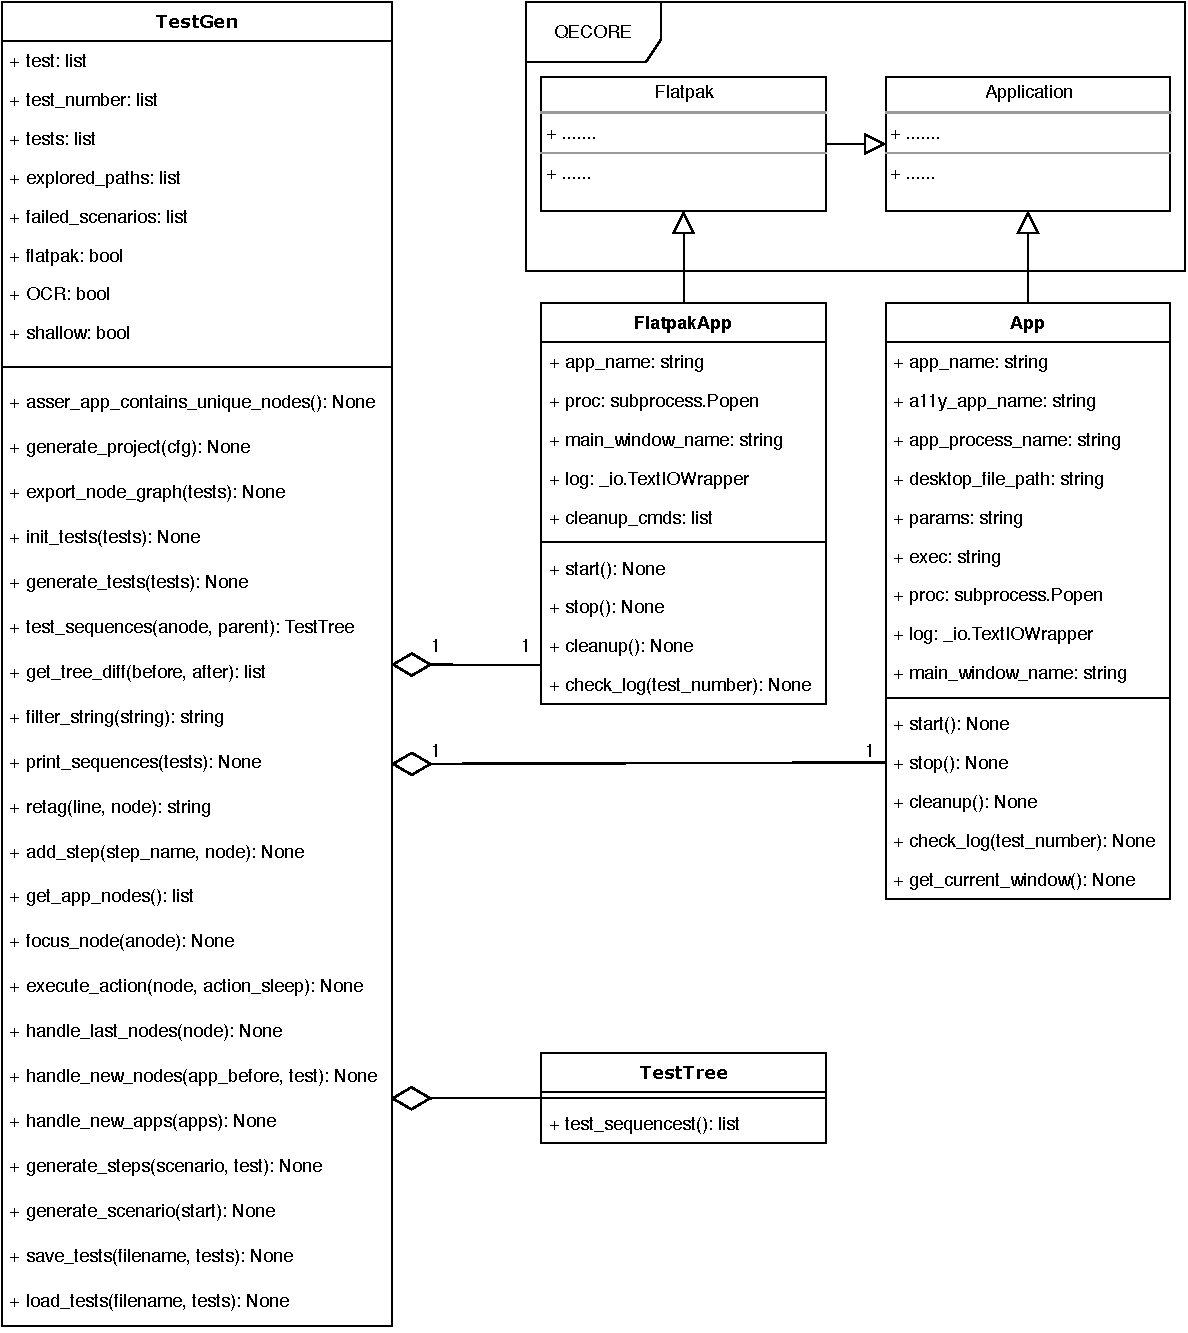
\includegraphics[width=1\textwidth,clip]{obrazky-figures/TestGen_class_diagram.pdf}
	\caption{Class diagram describing an overview over the implementation of the test generator}
	\label{test_gen}
\end{figure}

\section{Generation process}
The input to the test generator data about the tested application entered in the \texttt{apps.yaml} file. The output is a project structure containing generated test cases and other files required for test execution. The test generation process can be divided into multiple parts and is described throughout the next sections.

\subsection{Generating an Application Project and Setup}
Initially, the test generator checks the availability of the record about a tested application in the configuration file \texttt{apps.yaml}. Subsequently, it creates a sub-folder with the name of the application where generated content will be placed. Additionally, predefined source files with the implementation of steps (required by the behave framework) are copied to the folder structure with scripts and other files that are necessary for the test execution. The Figure \ref{project_folder} demonstrates the structure after the test generation. The folder features contains the test cases written in the file \texttt{generated.feature}. The file \texttt{environment.py} contains setup required for test execution, it imports the setup from the \texttt{qecore} library and creates an instance of either the \texttt{Flatpak} or the \texttt{Application}. The type of the application (flatpak or application) and the parameters for the class instance are extracted from the entry in the configuration file \texttt{apps.yaml}. The folder steps contains source files that implements the steps which are performed in the generated test cases. The module \texttt{ocr\_steps.py} contains only one behave step which should be used for the verification of the string on the screen. The module \texttt{steps.py} contains implementation of seven behave steps. Their decorators are written as generally as possible to keep the codebase minimal but still allow to execute any action, verify any state or check 

\begin{figure}[H]
\dirtree{%
.1 gnome-terminal.
.2 features.
.3 generated.feature.
.3 environment.py.
.3 steps.
.4 ocr\_steps.py.
.4 steps.py.
.2 gnome-terminal.log.
.2 mapper.yaml.
.2 requirements.txt.
.2 runtesh.sh.
}
\caption{Framing a dirtree-generated figure}
\label{project_folder}
\end{figure}

\subsection{Generating test cases}



\section{OCR integration}
The main goal of the OCR integration in this work is to provide an additional level of verification of string values presented by applications and thus not rely purely on AT-SPI. However, the integration of the OCR into generated test cases has to be reliable to avoid false-positive results from the tests. Therefore, the integration of Tesseract has to be properly tested and the implementation has to contain image preprocessing optimizations and configuration to achieve specified goals.
Tesseract offers several options that allow to optimize test detection and analysis. One of them is  the definition of the recognized language. It is assumed that most of the tested applications will use the English language and therefore, the dataset trained for the English language is used.

\subsection{Screenshot Preprocessing and Optimizations}
As discussed in \ref{OCR_section}, Tesseract is less prone to errors when operating with images containing black text on a white background. Therefore the safest option, is a conversion of images with thresholding to binary colors (black and white). It also has to be considered that some applications are using darker themes or contain parts with different color schemes. To avoid problems with text detection connected to this, the string is always searched in two images. The first one is a binarized copy of the original image, the second one is a copy of the binarized scale image with inverted colors. This ensures that the searched string is found on the screen, if present, regardless of a theme set in an application and prevents false-positive results during the test execution. An example is shown in Figure \ref{ocr_conversion}, containing 3 images, ordered from the top: an original image, a binarized image, and an inverted binarized image. The Listings \ref{OCR_text2} is showing the result of the character recognition when the image contains black text on a white background. The result contains almost all strings shown on the screen with some random characters created as an attempt to read icons located in the right top corner of the window. When compared to Listings \ref{OCR_text1}, where the source image contains white text on a black background, it proves an increase of the efficiency achieved after the optimization. The results obtained from the original image are quite similar to the results in Listing \ref{OCR_text1}. The conversion is implemented via \texttt{threshold} method from the OpenCV module.

\begin{figure}[H]
	\centering
	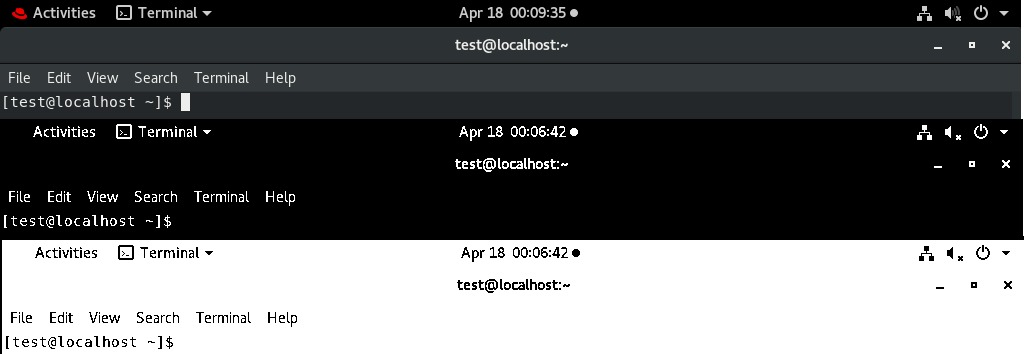
\includegraphics[width=1\textwidth,clip]{obrazky-figures/OCR_conversion.jpg}
	\caption{Steps of image preprocessing for Optical Character Recognition tool Tesseract, From the top: the original image, the binarized image, the inverted binarized image}
	\label{ocr_conversion}
\end{figure}

\begin{lstlisting}[caption={Text generated from the binarized image in Figure \ref{ocr_conversion}},label={OCR_text1}]
Pet) Terminal ~ EV ee muerre. Ty Pa) Ones
Peels ee?

Ca sa
[test@localhost ~]$ 
\end{lstlisting}
\begin{lstlisting}[caption={Text generated from the inverted binarized image in Figure \ref{ocr_conversion}},label={OCR_text2}]
 Activities Terminal ~ Apr 18 00:22:36 AO Orhttps://www.overleaf.com/project/5e92281e1d9c8a0001314a50
test@localhost:~ - 9 x

File Edit View Search Terminal Help
[test@localhost ~]$
\end{lstlisting}

Further experiments have shown additional issues with text formatting and recognition of certain letters. These facts lead to another set of  optimizations that were implemented to avoid false positive test cases. A search for a string containing multiple words with white spaces might fail because the result might not contain all the white-spaces. Strings containing symbols …, -, \_, and — could be easily exchanged during the recognition. Those letters are not as important as letters representing the actual text. Therefore, a search for a match in the extracted text is performed twice. The first attempt tries to match the string with white spaces and full formatting. If that attempt fails, the second attempt breaks the string into words and tries to match every word separately. The second attempt is also followed by a warning message that the string was not matched in the original version.

The Tesseract has shown occasional difficulties with recognition of similarly looking letters. The most affected character was \textbf{I} exchanged for \textbf{1}, followed by \textbf{S} exchanged for \textbf{5}. Despite these occasional cases, the implementation works quite reliably both during the test generation process and the execution process. Nevertheless, the time consumed by taking screenshots during the generation process is significant. Therefore, the developed tool has the ability to disable the generation of the OCR steps during the generation of test cases through the command line parameter \texttt{-{}-disable-OCR}. If the generated test cases already contain steps performing OCR checks and are intended to be executed without them, the tests can be executed with the shell variable \texttt{OCR=False}. The defined variable will cause skipping of the OCR checks, although they will still be shown in the test logs as executed. This is caused by the limitation of the behave framework as it only allows to skip whole test scenarios. The test results executed with the variable will contain a warning message about skipped OCR steps.

\subsection{Implemented Steps}
The results obtained from experiments with the OCR were implemented to a single behave step. The step contains a string variable that should be found on the screen at specific moment during the test execution. The process involves taking a screenshot via \texttt{gnome-screenshot} utility. It continues with image preprocessing and extraction of the text from two variants of images. Finally, an assertion is made to confirm the presence of the string on the screen. The Listing \ref{ocr_test} contains a test case generated for \textit{Gedit} flatpak, in this case the OCR should confirm the presence of the \textit{Save} button on the screen. The introduced optimizations from the last section should help to avoid false-positive results. However, if the OCR fails to find the string on the screen, the error message printed to a log will contain all the extracted text. This should help the testers with easier identification of false-positives.

\begin{lstlisting}[language=Gherkin,caption={Test case demonstrating the OCR integration in test cases},label={ocr_test}]
    @18_Save
    Scenario: org.gnome.gedit: 18_Save
      * Start: "org.gnome.gedit" via command in session
      * State: "push button" "Save" "showing" is "True"
      * OCR: "Save" is shown on the screen
      * Action: "click" "Save" "push button"
      * State: "file chooser" "Save As" is shown
\end{lstlisting}

\section{Test Execution}
The result of the generation process is a folder structure containing generated test cases, configuration files, and scripts for execution in the CI environment. Generated test cases are located in the file named \texttt{generated.feature}. The file contains all the test cases divided into so-called scenarios. Each scenario has a unique name starting with character \texttt{@}, thus allowing a single test execution if required. The test can be executed also at once by simply executing command \texttt{behave} in the generated project folder. The test are also respecting the cleanup commands which are set in \texttt{apps.yaml}. The cleanup is always executed after the finish of the test, regardless of the result of the executed tests. Behave either prints steps from a test scenario to standard output or can generate an HTML log. This log format is more suitable for examination of the results executed in the CI environment. Thanks to the setup done by the \textit{qecore} library, the test reports have embedded logs, videos from the test runs, and a screenshot generated in a moment, when the test case fails. 

% TODO. more on project structure
% An example of the generated test case scenario is available ....

\chapter{Testing en results}
test coverage, node coverage, action coverage




\chapter{Conclusion}
